\documentclass[12pt, aspectratio = 169, xcolor = x11names]{beamer}
\title[CiSS]{%
  Context-Reinforced Semantic Segmentation\\
  CiSS
}
\author[Freed Wu]{Speaker: Freed Wu}
\institute[USTC]{%
  Electronic Engineering and Information Science\\
  University of Science and Technology of China
}
\date{\today}
\AtBeginSection[]{%
  \setbeamertemplate{footline}[footlineoff]
  \begin{frame}
    \frametitle{Contents}
    \tableofcontents[currentsection,subsectionstyle=show/show/hide]
  \end{frame}
  \setbeamertemplate{footline}[footlineon]
}
\AtBeginSubsection[]{%
  \setbeamertemplate{footline}[footlineoff]
  \begin{frame}
    \frametitle{Contents}
    \tableofcontents[currentsection,subsectionstyle = show/shaded/hide]
  \end{frame}
  \setbeamertemplate{footline}[footlineon]
}
\graphicspath{{fig/}}
\usepackage[ustcblue]{ustcbeamer}
\usepackage{qrcode}
\usepackage{fontawesome5}
\usepackage{subcaption}
\usepackage{bbm}
\usepackage{csvsimple}
\usepackage{booktabs}
\usepackage[ruled, vlined]{algorithm2e}
\usepackage{physics}
\begin{document}

\maketitleframe%
\begin{frame}
  \frametitle{Contents}
  \tableofcontents[hideallsubsections]
\end{frame}

\section{Introduction}%
\label{sec:introduction}

\begin{frame}
  \frametitle{Main object}
  P-map has encoded a large number of contextual information not only local
  (e.g.\ objects) but also global (e.g.\ layout).

  Hence, the paper proposes a new model named CiSS to explore the p-map to
  generate another source of scene context which can be effectively combined
  with traditional features.
\end{frame}

\begin{frame}
  \frametitle{CiSS v.s. CFN}
  \begin{figure}[htbp]
    \centering
    \begin{subfigure}[htbp]{0.22\linewidth}
      \centering
      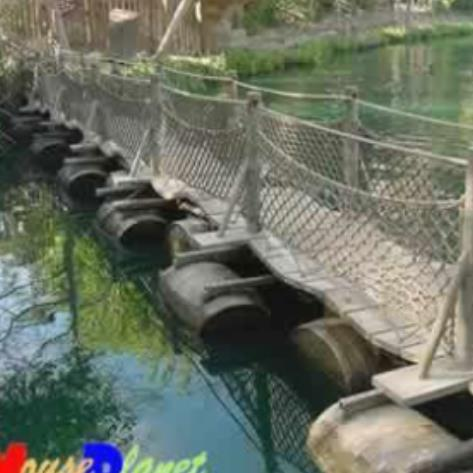
\includegraphics[
      width = \linewidth,
      ]{input}
      \caption{Input}%
      \label{fig:input}
    \end{subfigure}
    \quad
    \begin{subfigure}[htbp]{0.22\linewidth}
      \centering
      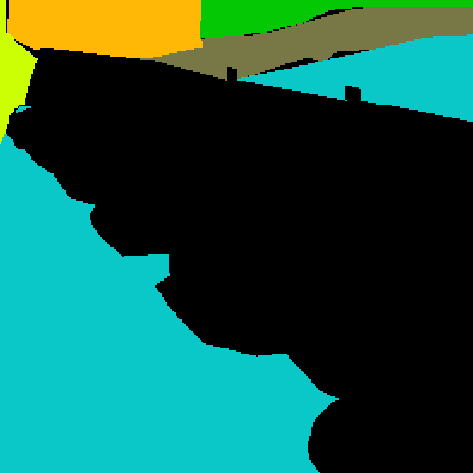
\includegraphics[
      width = \linewidth,
      ]{truth}
      \caption{Ground truth}%
      \label{fig:truth}
    \end{subfigure}
    \quad
    \begin{subfigure}[htbp]{0.22\linewidth}
      \centering
      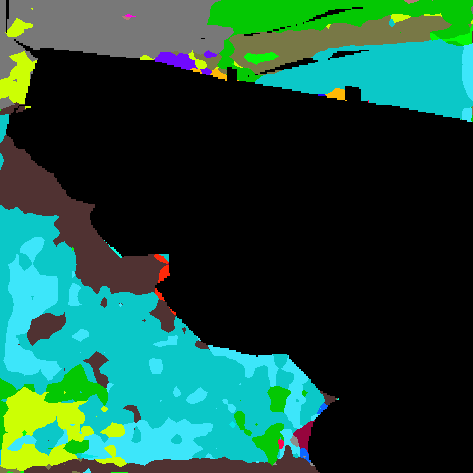
\includegraphics[
      width = \linewidth,
      ]{cfn}
      \caption{CFN}%
      \label{fig:cfn}
    \end{subfigure}
    \quad
    \begin{subfigure}[htbp]{0.22\linewidth}
      \centering
      
\includegraphics[
      width = \linewidth,
      ]{ciss}
      \caption{CiSS}%
      \label{fig:ciss}
    \end{subfigure}
    \caption{Compare}%
    \label{fig:compare}
  \end{figure}

  \pause%
  \alert{Notice deceiving reflection of trees in the water!}
\end{frame}

\begin{frame}
  \frametitle{Evaluate index}
  \begin{columns}
    \begin{column}{0.5\textwidth}
      A evaluate index $I$ should statisfy the following conditions:
      \pause%
      \begin{itemize}[<+->]
        \item$0 \leqslant I \leqslant 1$ and
          \begin{itemize}
            \item$I = 0$ iff $A_\mathrm{pred} \cap A_\mathrm{true} = \emptyset$
            \item$I = 1$ iff $A_\mathrm{pred} = A_\mathrm{true}$
          \end{itemize}
        \item$\lvert A_\mathrm{pred} \cap A_\mathrm{true}\rvert \uparrow, I \uparrow$
      \end{itemize}
    \end{column}
    \pause%
    \begin{column}{0.5\textwidth}
      \begin{definition}[mIoU]
        Mean of intersection over union.
        \begin{align*}
          \mathrm{IoU} = \frac{\lvert A_\mathrm{pred} \cap A_\mathrm{true}\rvert}{\lvert A_\mathrm{pred} \cup A_\mathrm{true}\rvert}
        \end{align*}
      \end{definition}
      \pause%
      \begin{definition}[dice coeffience]
        \begin{align*}
          \mathrm{Dice} = \frac{2\lvert A_\mathrm{pred} \cap A_\mathrm{true}\rvert}{\lvert A_\mathrm{pred}\rvert + \lvert A_\mathrm{true}\rvert}
        \end{align*}
      \end{definition}
    \end{column}
  \end{columns}
\end{frame}

\begin{frame}
  \frametitle{Evaluate index}
  \begin{columns}
    \begin{column}{0.5\textwidth}
      \begin{block}{Quantize}
        \begin{align*}
          \lvert A_\mathrm{pred} \cap A_\mathrm{true}\rvert = & \sum M_\mathrm{pred} \cdot M_\mathrm{true}\\
          \lvert A_\mathrm{pred}\rvert = & \sum\sqrt{M_\mathrm{pred} \cdot M_\mathrm{pred}}
        \end{align*}
        \begin{itemize}
          \item$\cdot$ means element-wise multiplication.
          \item$\sqrt{}$ means element-wise square root.
          \item$\sum$ means summarization of elements of a matrix.
        \end{itemize}
      \end{block}
    \end{column}
    \begin{column}{0.5\textwidth}
      \begin{definition}[mIoU]
        Mean of intersection over union.
        \begin{align*}
          \mathrm{IoU} = \frac{\lvert A_\mathrm{pred} \cap A_\mathrm{true}\rvert}{\lvert A_\mathrm{pred} \cup A_\mathrm{true}\rvert}
        \end{align*}
      \end{definition}
      \begin{definition}[dice coeffience]
        \begin{align*}
          \mathrm{Dice} = \frac{2\lvert A_\mathrm{pred} \cap A_\mathrm{true}\rvert}{\lvert A_\mathrm{pred}\rvert + \lvert A_\mathrm{true}\rvert}
        \end{align*}
      \end{definition}
    \end{column}
  \end{columns}
\end{frame}

\section{Model}%
\label{sec:model}

\subsection{Framework}%
\label{sub:framework}

\begin{frame}
  \frametitle{Framework}
  \begin{columns}
    \begin{column}{0.45\textwidth}
      \begin{figure}[htbp]
        \centering
        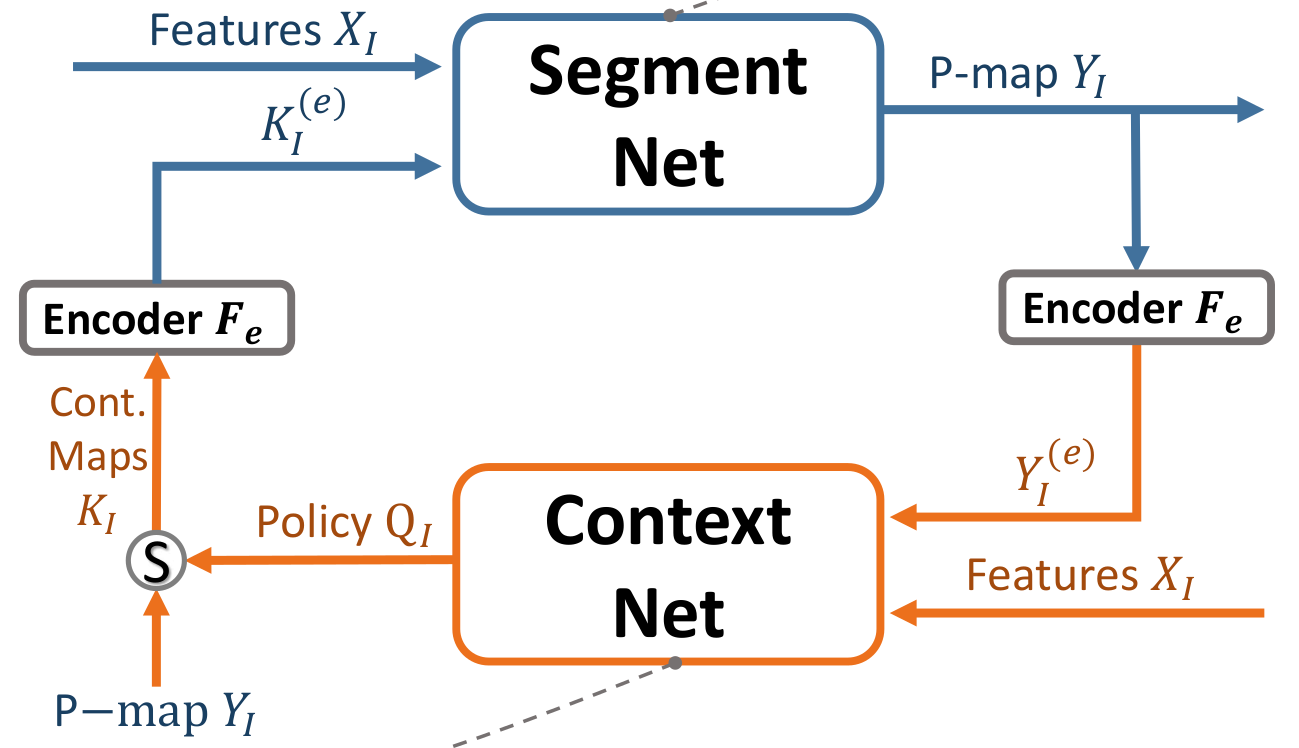
\includegraphics[
          width = 0.8\linewidth,
        ]{framework}
        \caption{Framework}%
        \label{fig:framework}
      \end{figure}
    \end{column}
    \pause%
    \begin{column}{0.55\textwidth}
      \begin{description}[<+->]
        \item[Domain features]$X_I \in \mathbb{R}^{H' \times W' \times C}$
        \item[Context map]$K_I \in \mathbb{Z}_{N_\mathrm{c}}^{H' \times W'}$
        \item[P-map]$Y_I \in \mathbb{R}^{H^\circ \times W^\circ}$
        \item[Encoded context map]$K_I^{(\mathrm{e})} \in \mathbb{R}^{H'
          \times W' \times C_\mathrm{e}}$
        \item[Encoded p-map]$Y_I^{(\mathrm{e})} \in \mathbb{R}^{H^\circ
          \times W^\circ \times C_\mathrm{e}}$
        \item[Policy]$Q_I \in \mathbb{R}^{H^\circ \times W^\circ \times 2}$
      \end{description}
    \end{column}
  \end{columns}
\end{frame}

\begin{frame}
  \frametitle{Framework}
  \begin{columns}
    \begin{column}{0.45\textwidth}
      \begin{itemize}[<+->]
        \item$K_I(i, j) = 0$ means classification label is uncertain.
        \item$H^\circ \neq H', W^\circ \neq W'$ due to resolution
          degradation.
        \item$Q_I(i, j, 1)$ denotes the action of adopting the prediction
          $Y_I(i, j)$, whereas $Q_I(i, j, 0)$ ignores the prediction.
        \item<+-|alert@+>End-to-end design $F_\mathrm{s} \rightarrow
          F_\mathrm{e} \rightarrow F_\mathrm{k} \rightarrow
          F_\mathrm{e} \rightarrow F_\mathrm{s}$.
      \end{itemize}
    \end{column}
    \begin{column}{0.55\textwidth}
      \begin{description}
        \item[Domain features]$X_I \in \mathbb{R}^{H' \times W' \times C}$
        \item[Context map]$K_I \in \mathbb{Z}_{N_\mathrm{c}}^{H' \times W'}$
        \item[P-map]$Y_I \in \mathbb{R}^{H^\circ \times W^\circ}$
        \item[Encoded context map]$K_I^{(\mathrm{e})} \in \mathbb{R}^{H'
          \times W' \times C_\mathrm{e}}$
        \item[Encoded p-map]$Y_I^{(\mathrm{e})} \in \mathbb{R}^{H^\circ
          \times W^\circ \times C_\mathrm{e}}$
        \item[Policy]$Q_I \in \mathbb{R}^{H^\circ \times W^\circ \times 2}$
      \end{description}
    \end{column}
  \end{columns}
\end{frame}

\begin{frame}
  \frametitle{Encoder}
  \begin{columns}
    \begin{column}{0.5\textwidth}
      \begin{figure}[htbp]
        \centering
        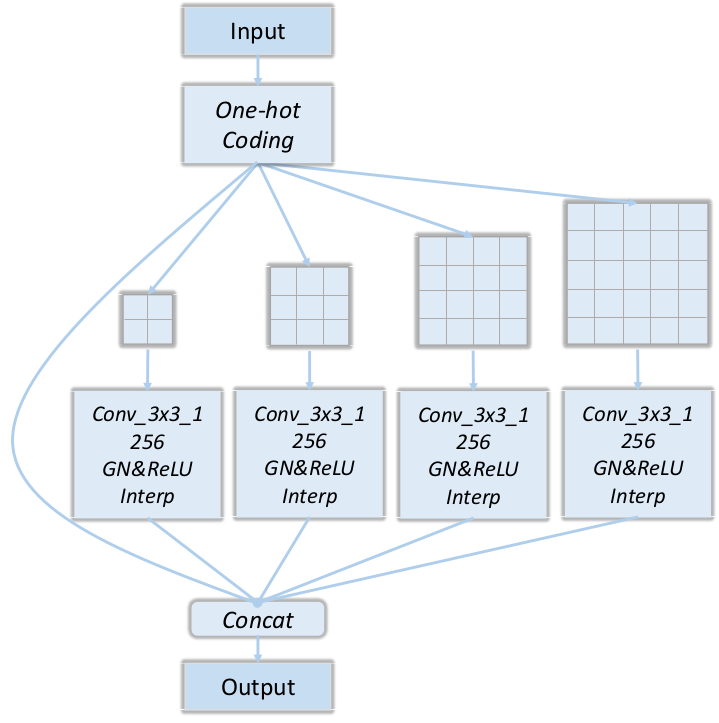
\includegraphics[
          width = 0.8\linewidth,
        ]{encoder}
        \caption{Encoder}%
        \label{fig:encoder}
      \end{figure}
    \end{column}
    \pause%
    \begin{column}{0.5\textwidth}
      \begin{itemize}[<+->]
        \item$K_I^\mathrm{(e)} = F_\mathrm{e}(K_I)$
        \item<+-|alert@+>Context is high-level information which shouldn't be
          confused with other low-level information (e.g.\ texture,
          boundaries).
      \end{itemize}
    \end{column}
  \end{columns}
\end{frame}

\subsection{Segment Net}%
\label{sub:segment_net}

\begin{frame}
  \frametitle{S-Net}
  \begin{columns}
    \begin{column}{0.5\textwidth}
      \begin{figure}[htbp]
        \centering
        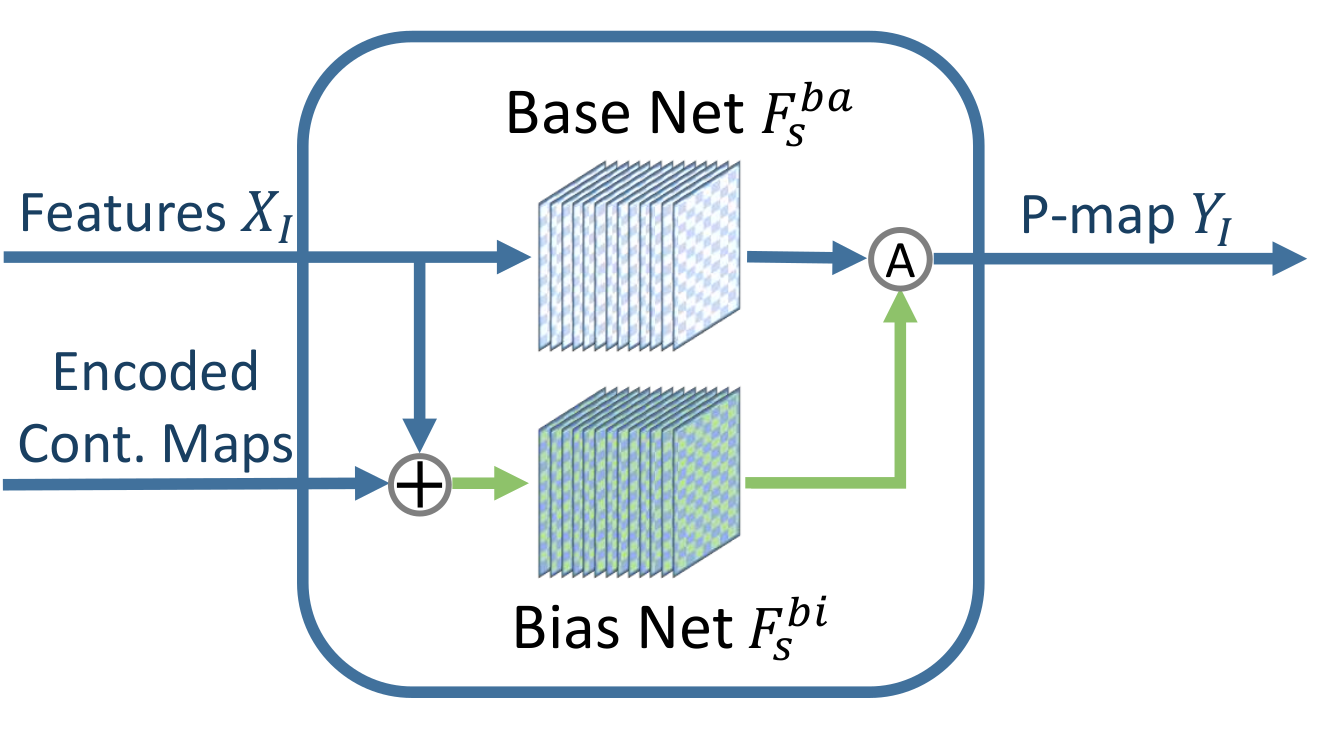
\includegraphics[
          width = 0.8\linewidth,
        ]{snet}
        \caption{S-Net}%
        \label{fig:snet}
      \end{figure}
    \end{column}
    \pause%
    \begin{column}{0.5\textwidth}
      \begin{itemize}[<+->]
        \item$Y_I = F_\mathrm{s}(X_I, K_I) = F_\mathrm{s}^\mathrm{ba}(X_I) +
          F_\mathrm{s}^\mathrm{bi}(X_I \oplus K_I^{(\mathrm{e})})$
        \item Initially, $K_I^{(\mathrm{e})}$ is none,
          $F_\mathrm{s}^\mathrm{bi}$ will return 0.
        \item Base net has 2 convolutional layers which channel, stride, and
          kernel size are 512, 1, and 3 respectively.
        \item Bias net uses the same architecture as C-Net except a little
          modification to fit input/output dimension.
      \end{itemize}
    \end{column}
  \end{columns}
\end{frame}

\subsection{Context Net}%
\label{sub:context_net}

\begin{frame}
  \frametitle{C-Net}
  \begin{columns}
    \begin{column}{0.5\textwidth}
      \begin{figure}[htbp]
        \centering
        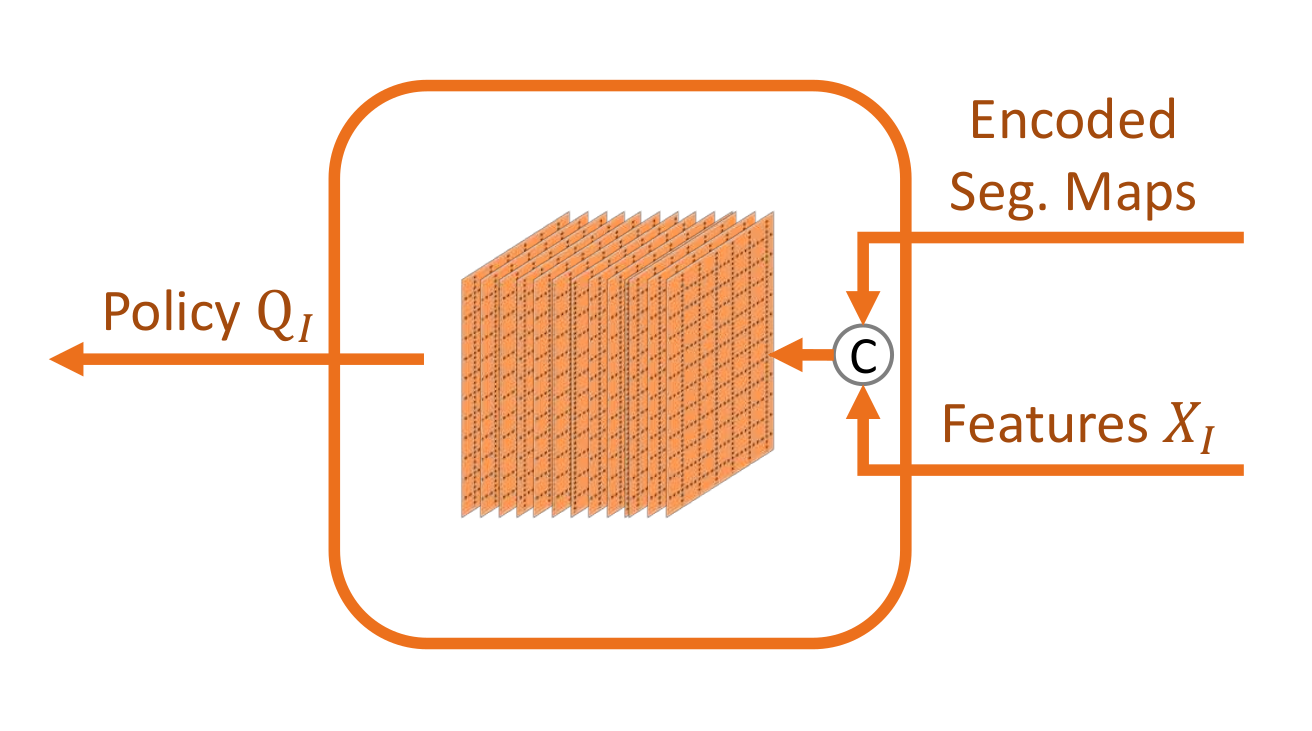
\includegraphics[
          width = 0.8\linewidth,
        ]{cnet}
        \caption{C-Net}%
        \label{fig:cnet}
      \end{figure}
    \end{column}
    \pause%
    \begin{column}{0.5\textwidth}
      \begin{itemize}[<+->]
        \item$Q_I = F_\mathrm{k}(X_I \oplus Y_I^{(\mathrm{e})})$
        \item 5-layer CNN
      \end{itemize}
    \end{column}
  \end{columns}
\end{frame}

\begin{frame}
  \frametitle{C-Net}
  \begin{columns}
    \begin{column}{0.5\textwidth}
      \begin{figure}[htbp]
        \centering
        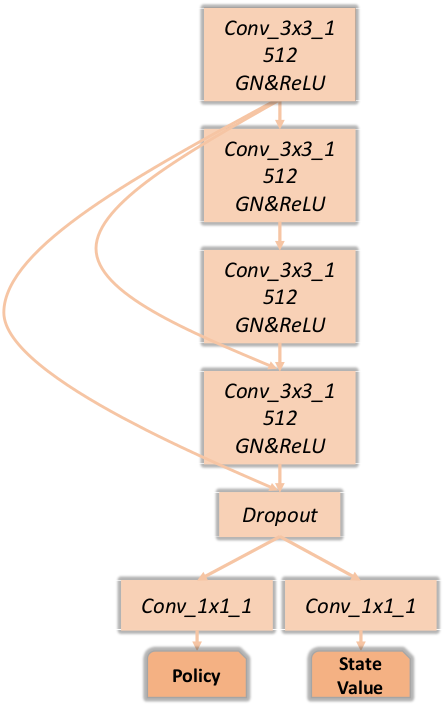
\includegraphics[
          width = 0.6\linewidth,
        ]{architecture}
        \caption{Architecture}%
        \label{fig:architecture}
      \end{figure}
    \end{column}
    \begin{column}{0.5\textwidth}
      \begin{itemize}
        \item$Q_I = F_\mathrm{k}(X_I \oplus Y_I^{(\mathrm{e})})$
        \item 5-layer CNN
      \end{itemize}
    \end{column}
  \end{columns}
\end{frame}

\begin{frame}
  \frametitle{MDP}
  \begin{columns}
    \begin{column}{0.48\textwidth}
      \begin{figure}[htbp]
        \centering
        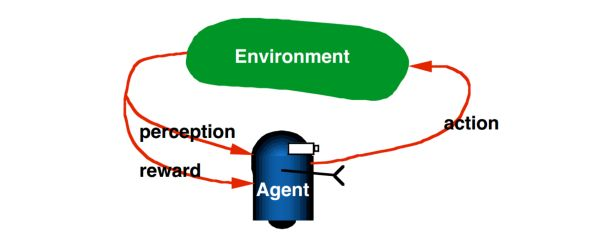
\includegraphics[
          width = 0.8\linewidth,
        ]{mdp}
        \caption{Markov Decision Process}%
        \label{fig:mdp}
      \end{figure}
    \end{column}
    \pause%
    \begin{column}{0.52\textwidth}
      \begin{definition}[MDP]
        a tuple $(S, A, P, r)$, where
      \end{definition}
      \pause%
      \begin{description}[<+->]
        \item[$S$]State space (i.e.\ a set containing all states of the
          environment.)
        \item[$A$]Action space (i.e.\ a set containing all actions of the agent.)
        \item[$P$]$S \times A \times S \rightarrow [0, 1]$ Transition
          probability distribution.
        \item[$r$]$S \times A \rightarrow \mathbb{R}$ Reward function.
      \end{description}
    \end{column}
  \end{columns}
\end{frame}

\begin{frame}
  \frametitle{MDP}
  \begin{columns}
    \begin{column}{0.48\textwidth}
      In this model, P-net and C-net are environment and agent respectively.
      \begin{description}[<+->]
        \item[$S$]$\{Y_I\}$.
        \item[$A$]$\{B_I\} = \mathbb{Z}_2^{H^\circ \times W^\circ}$.
          \begin{align*}
            P(B_I(i, j) = k) = & Q_I(i, j, k)\\
            k \in & \mathbb{Z}_2
          \end{align*}
      \end{description}
    \end{column}
    \begin{column}{0.52\textwidth}
      \begin{definition}[MDP]
        a tuple $(S, A, P, r)$, where
      \end{definition}
      \begin{description}
        \item[$S$]State space (i.e.\ a set containing all states of the
          environment.)
        \item[$A$]Action space (i.e.\ a set containing all actions of the
          agent.)
        \item[$P$]$S \times A \times S \rightarrow [0, 1]$ Transition
          probability distribution.
        \item[$r$]$S \times A \rightarrow \mathbb{R}$ Reward function.
      \end{description}
    \end{column}
  \end{columns}
\end{frame}

\begin{frame}
  \frametitle{MDP}
      \begin{description}[<+->]
        \item[$P$]A deterministic environment.
          \begin{align*}
            P(Y_{I(t + 1)} = F_\mathrm{s}(X_{I(t)}, K_{I(t)})\mid Y_{I(t)}) =
            1\\
          \end{align*}
          where
          \begin{align*}
            K_{I(t)} = & (Y_{I(t)} + 1) \cdot B_{I(t)}
          \end{align*}
      \end{description}
\end{frame}

\begin{frame}
  \frametitle{MDP}
  \begin{description}
    \item[$r$]$L_I$ is the label of ground truth.
  \end{description}
  \begin{align*}
    r(t) = & \beta_1\mathbbm{1}_{K_{I(t)}(i, j) = L_{I(t)}(i, j)} +
    \beta_2\mathbbm{1}_{K_{I(t)}(i, j) = 0}\\
    + & \frac{1}{C_\mathrm{h}C_\mathrm{w}} \sum_{%
      i' \in [i - \frac{C_\mathrm{h}}{2}, i + \frac{C_\mathrm{h}}{2}],
      j' \in [j - \frac{C_\mathrm{w}}{2}, j + \frac{C_\mathrm{w}}{2}]
    }M(
    \mathbbm{1}_{Y_{I(t)}(i', j') = L_{I(t)}(i', j')},
    \mathbbm{1}_{Y_{I(t + 1)}(i', j') = L_{I(t)}(i', j')}
    )
  \end{align*}
  where

  \begin{center}
    $M(x, y) =
    \begin{cases}
      0, (x, y) = (0, 0)\\
      1, (x, y) = (0, 1)\\
      -1, (x, y) = (1, 0)\\
      0.5, (x, y) = (1, 1)
    \end{cases}$
  \end{center}
\end{frame}

\begin{frame}
  \frametitle{MDP}
  The aim of MDP is to maximize the expected discount reward $\eta$.

  \begin{center}
    max $\eta = \mathbb{E}_{s_0, a_0, s_1, a_1, \ldots} \sum^\infty_{t = 0} \gamma^t r_t$

    s.t.$
    \begin{cases}
      s_0 \sim \rho_0\\
      a_t \sim \pi(a_t \mid s_t)\\
      s_{t + 1} \sim P(s_{t + 1}|s_t)
    \end{cases}$
  \end{center}

  where $\gamma \in \left(0, 1\right]$ is a constant.
\end{frame}

\subsection{Asynchronous Advantage Actor-Critic Algorithm}%
\label{sub:asynchronous_advantage_actor-critic_algorithm}

\begin{frame}
  \frametitle{Advantage function}
  \begin{align*}
    V(s_t) = & \mathbb{E}_{a_t, s_{t + 1}, a_{t + 1}, s_{t + 2}, \ldots}\sum^\infty_{l = 0} \gamma^l r_{t + l}\\
    Q(s_t, a_t) = & \mathbb{E}_{s_{t + 1}, a_{t + 1}, s_{t + 2}, s_{t + 2}, \ldots}\sum^\infty_{l = 0} \gamma^l r_{t + l}\\
    A(s_t, a_t) = & Q(s_t, a_t) - V(s_t)\\
    A_k(s_t, a_t) = & \mathbb{E}_{s_{t + 1}, a_{t + 1}, s_{t + 2}, s_{t + 2}, \ldots, a_{t + k}}\sum^{k - 1}_{l = 0} \gamma^l r_{t + l} + \gamma^k V(s_{t + k}) - V(s_t)\\
    \lim_{k \rightarrow \infty}A_k(s_t, a_t) = & A(s_t, a_t)\\
    \eta = & V(s_0)
  \end{align*}
\end{frame}

\begin{frame}
  \frametitle{A3C}
  \begin{algorithm}[H]
    \caption{Asynchronous Advantage Actor Critic Algorithm}%
    \label{al:asynchronous_advantage_actor_critic_algorithm}
    \tiny
    \KwIn{global shared parameter vectors $\theta, \theta_\mathrm{v}$, thread specific parameter vectors $\theta', \theta'_\mathrm{v}$}
    \KwData{global shared counter $T = 0$, thread step counter $t = 1$}
    \While{$T < T_{\max}$}{%
      $\dd{\theta}, \dd{\theta_\mathrm{v}} = 0$\;
      $\theta' = \theta$\;
      $\theta'_\mathrm{v} = \theta_\mathrm{v}$\;
      $t_\mathrm{start} = t$\;
      $s = s_t$\;
      \While{$s_t$ is not terminal $t - t_\mathrm{start} < t_{\max}$}{%
        Simulate acton $a_t$ according to $\pi(a_t\mid s;\theta)$\;
        Receive reward $r_t$ and next state $s_{t + 1}$\;
        t++\;
        T++\;
      }
      \eIf{$s_t$ is terminal}{%
        $R = 0$\;
        }{%
        $R = V(s_t, \theta'_\mathrm{v})$\;
      }
      \For{$i = t - 1; i \geqslant t_\mathrm{start}; i--$}{%
        $R = r_i + \gamma R$\;
        $\dd{\theta} = \dd{\theta} + \nabla_{\theta'}\log \Bigl(\pi(a_i\mid s_i; \theta')\bigl(R-V(s_i; \theta'_\mathrm{v})\bigr)\Bigr)$\;
        $\dd{\theta_\mathrm{v}} = \dd{\theta_\mathrm{v}} + \pdv{}{\theta'_\mathrm{v}}\relax{\bigl(R - V(s_i; \theta'_\mathrm{v})\bigr)}^2$\;
      }
      $\theta = \theta + \dd{\theta}$\;
      $\theta_\mathrm{v} = \theta + \dd{\theta_\mathrm{v}}$\;
    }
  \end{algorithm}
\end{frame}

\begin{frame}
  \frametitle{Loss function}
  \begin{columns}
    \begin{column}{0.5\textwidth}
      \begin{figure}[htbp]
        \centering
        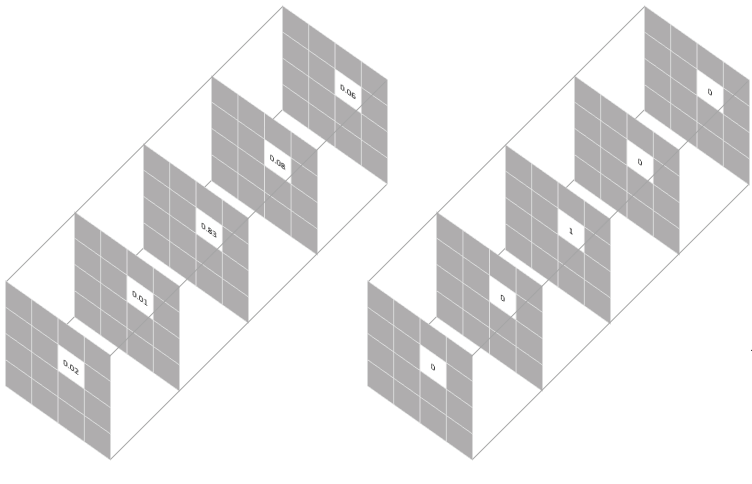
\includegraphics[
          width = 0.8\linewidth,
        ]{loss}
        \caption{Loss}%
        \label{fig:loss}
      \end{figure}
      Loss function is used to evaluate the difference between prediction and
      ground truth label.
      Well-designed loss function can help model converge fast.
    \end{column}
    \pause%
    \begin{column}{0.5\textwidth}
      \begin{definition}[Mean square error, L2]
        $\mathrm{MSE} = \frac{1}{N}\sum_{i, j} {(L(i, j) - Y(i, j))}^2$
      \end{definition}
      \pause%
      \begin{definition}[Mean absolute error, L1]
        $\mathrm{MAE} = \frac{1}{N}\sum_{i, j} \lvert L(i, j) - Y(i, j)\rvert$
      \end{definition}
      \pause%
      \begin{definition}[cross entropy loss]
        Cross entropy loss is closer to the sensitivity of human eyes than
        above 2 pixel-wise loss function.
        $\mathrm{Loss}_\mathrm{s} = -\sum_{i, j} L(i, j)\log Y(i, j)$
      \end{definition}
    \end{column}
  \end{columns}
\end{frame}

\begin{frame}
  \frametitle{Loss function}
  \begin{align*}
    \mathrm{Loss} = & \mathrm{Loss}_\mathrm{p} + \mathrm{Loss}_\mathrm{v} + \lambda_1\mathrm{Loss}_\mathrm{s} + \lambda_2\mathrm{Loss}_\mathrm{e}\\
    \mathrm{Loss}_\mathrm{p} = & \log \bigl(\pi(a_t\mid s_t; \theta_k)\bigr)A(a_t, s_t)\\
    \mathrm{Loss}_\mathrm{v} = & {\bigl(R - V(s_t; \theta_\mathrm{v})\bigr)}^2\\
    \mathrm{Loss}_\mathrm{e} = & \pi\log\pi
  \end{align*}
\end{frame}

\section{Experiment}%
\label{sec:experiment}

\subsection{Dataset}%
\label{sub:dataset}

\begin{frame}
  \frametitle{Dataset}
  \begin{description}
    \item[\href{http://groups.csail.mit.edu/vision/datasets/ADE20K/}{ADE20K}]20k train, 2k validation, 3k test.
    \item[\href{https://www.cityscapes-dataset.com/}{cityscapes}]Dataset of semantic urban scene understanding from 50 cities.
    \item[\href{https://www.cs.stanford.edu/~roozbeh/pascal-context/}{pascal-context}]Indoor and outdoor scenes with 400+ classes.
  \end{description}
\end{frame}

\subsection{Implement}%
\label{sub:implement}

\begin{frame}
  \frametitle{Implement}
  \begin{enumerate}[<+->]
    \item Initially, generate $X_I$ as basebone by PSPNet pre-trained on the
      three datasets.
    \item Implement CiSS with Tensorflow and 16 Nvidia M40 GPUs.
    \item Initial learning rates, then employ stochastic gradient descend.
  \end{enumerate}
\end{frame}

\subsection{Sensitivity Analysis}%
\label{sub:sensitivity_analysis}

\begin{frame}
  \frametitle{Sensitivity analysis}
  Adjust parameters to analysis variety. Keep $\lambda_1 = 1$.
  \begin{table}[htbp]
    \centering
    \caption{Sensitivity analysis}%
    \label{tab:sensitivity_analysis}
    \begin{subtable}[htbp]{0.45\linewidth}
      \centering
      \caption{$\gamma$}%
      \label{tab:gamma}
      \tiny
      \csvautobooktabular{tab/gamma.csv}
    \end{subtable}
    \quad
    \begin{subtable}[htbp]{0.45\linewidth}
      \centering
      \caption{$\beta_2$}%
      \label{tab:beta}
      \tiny
      \csvautobooktabular{tab/beta.csv}
    \end{subtable}
  \end{table}
  \pause%
  \begin{align*}
    \gamma \uparrow, \mathrm{IoU} \uparrow\\
    \beta_2 \uparrow, \mathrm{IoU} \uparrow
  \end{align*}
\end{frame}

\begin{frame}
  \frametitle{Sensitivity analysis}
  Regretfully, the training does not converge well when $\lambda > 0.15$,
  which infers that a balance between convergence and efficiency is crucial.
\end{frame}

\subsection{Ablation Study}%
\label{sub:ablation_study}

\begin{frame}
  \frametitle{Ablation study}
  \begin{table}[htbp]
    \centering
    \caption{RL strategy}%
    \label{tab:rl_strategy}
    \tiny
    \csvautobooktabular{tab/rl.csv}
  \end{table}
  Directly input p-map to S-Net is worse than baseline.
  CiSS outperforms others.
\end{frame}

\begin{frame}
  \frametitle{Ablation study}
  \begin{table}[htbp]
    \centering
    \caption{Iteration steps}%
    \label{tab:iteration_steps}
    \tiny
    \csvautobooktabular{tab/iteration.csv}
  \end{table}
  \begin{align*}
    t \uparrow, \mathrm{IoU} \uparrow
  \end{align*}
  The improvement becomes marginal as the iteration continues.
  Thus $t = 2$ is a trade-off between performance and time-complexity of
  inference.
\end{frame}

\subsection{Comparison}%
\label{sub:comparison}

\begin{frame}
  \frametitle{Comparison}
  \begin{table}[htbp]
    \centering
    \caption{Comparison}%
    \label{tab:comparison}
    \begin{subtable}[htbp]{0.32\linewidth}
      \centering
      \caption{ade20k}%
      \label{tab:ade20k}
      \tiny
      \setlength\tabcolsep{1pt}
      \csvautobooktabular{tab/ade20k.csv}
    \end{subtable}
    \begin{subtable}[htbp]{0.32\linewidth}
      \centering
      \caption{cityscapes}%
      \label{tab:cityscapes}
      \tiny
      \setlength\tabcolsep{1pt}
      \csvautobooktabular{tab/cityscapes.csv}
    \end{subtable}
    \begin{subtable}[htbp]{0.32\linewidth}
      \centering
      \caption{pascal-context}%
      \label{tab:pascal-context}
      \tiny
      \setlength\tabcolsep{1pt}
      \csvautobooktabular{tab/pascal-context.csv}
    \end{subtable}
  \end{table}
\end{frame}

\subsection{Discussion}%
\label{sub:discussion}

\begin{frame}
  \frametitle{Discussion}
  \begin{itemize}[<+->]
    \item The information in the learned context map is selected to have
      long-term benefits to the segmentation. (e.g.\ the reflection of trees
      on the water)
    \item Most of the contextual information is background objects and stuff,
      which proves that this kind of contextual information contains the
      overall layout of the scene that has rich sementic cues.
    \item The uncertain class is helpful in identifying the hard examples or
      high ambiguity reions in semantic segmentation.
  \end{itemize}
\end{frame}

\section{Conclusion}%
\label{sec:conclusion}

\begin{frame}
  \frametitle{Advantages}
  \begin{block}{Advantages}
    \pause%
    \begin{description}[<+->]
      \item[Innovation]Leverage p-map as source of contextual information.
      \item<+-|alert@+>[None]Good idea is enough. Others are minor.
    \end{description}
  \end{block}
\end{frame}

\begin{frame}
  \frametitle{Disadvantages}
  \begin{block}{Disadvantages}
    \pause%
    \begin{description}[<+->]
      \item[Subjectivity]e.g.\ the expression of reward function.
      \item[Difficulty]More parameters, more intractable on adjusting parameters.
      \item[Computationally expensive]And also expensive for money:)
    \end{description}
  \end{block}
\end{frame}

\begin{frame}
  \frametitle{Thanks}
  \begin{center}
    {\Large Thanks for your patience!}

    Click \href{https://github.com/Freed-Wu/ciss-beamer}{\faGithub} or scan
    \qrcode{https://github.com/Freed-Wu/ciss-beamer} to download this beamer.
  \end{center}

  \begin{flushright}
    Powered by \LaTeX.
  \end{flushright}
\end{frame}

\end{document}
